\documentclass[12pt, a4paper, bibliography=totoc]{scrartcl}

% personal data
\date{\today}


% language
\usepackage{polyglossia}
\setmainlanguage{english}
\setotherlanguages{german}
\usepackage{microtype}
\usepackage{dcolumn}

\usepackage[style=numeric,
			natbib=true,
			backend=biber]{biblatex}		%Bibliographie
\usepackage[autostyle=true,
			 german=quotes]
			 {csquotes}					%Anführungszeichen
\usepackage{blindtext}


%math and theorems
\usepackage{amsmath}
\usepackage{amssymb}
\usepackage{amsopn}					%Matheoperatoren
\usepackage[amsmath,thmmarks,hyperref]{ntheorem}
\usepackage{mathtools}
\usepackage{mathdots}					%Punkte
\usepackage{dsfont}
\usepackage{upgreek}					%Griechische Buchstaben
\usepackage{bbm}						%Mengensymbol
\usepackage{physics}					%Physiksymbole
\usepackage{relsize}						%Größenangaben
\usepackage[separate-uncertainty,
			per-mode=symbol]
			{siunitx}					%Einheiten
%\usepackage{tikz}						%Zeichnen
\usepackage{upgreek}					%Griechische Buchstaben
\usepackage{enumitem}
\setlist{nolistsep}


%useful packages
%\usepackage{geometry}
\usepackage{xcolor}
\usepackage{graphicx}
\usepackage{float}
\usepackage{csquotes}
\usepackage{todonotes}
\usepackage{booktabs}
\usepackage{array}
\usepackage[labelfont=bf]{caption}
\usepackage{wrapfig}
\usepackage{enumitem}
%\usepackage{xr} % cross referencing
%\usepackage{titling}
%\usepackage{titlesec}
%\usepackage[Bjornstrup]
%			{fncychap}					%Kapitellayout


\setmainfont{Linux Libertine O}
\setsansfont{Linux Biolinum O}

\usepackage{scrhack}					%Verbesserung Pakete
\usepackage{xltxtra}						%fontec


\newcommand{\im}{\mathrm{i}}
\newcommand{\e}{\mathrm{e}}
\renewcommand{\pi}{\uppi}
\renewcommand{\epsilon}{\varepsilon}


\addbibresource{bibliography.bib}

%color settings
\definecolor{myred}{RGB}{196,19,47} 
\definecolor{myblue}{RGB}{0,139,139}


%appendix
\usepackage[toc,page]{appendix}

%killing indent
\setlength{\parindent}{0pt}
\usepackage{multicol}
\usepackage{siunitx}
\usepackage{hyperref}


\title{Studying the $Z$ Boson with the ATLAS Detector at the LHC}
\author{Aaron Mielke \& Thomas Ackermann}
\date{\today}

\begin{document}

\begin{center}
	\makeatletter
	\thispagestyle{empty}
	
	\begin{figure}[H]
	\flushright
	
\includegraphics[width=0.35\textwidth]{fig/logo}
	\end{figure}
	
	\vspace{-30mm}
	
	\begin{flushleft}
	\large{\textbf{Fortgeschrittenen Praktikum} \\
		Summer term 2019} \\
	\end{flushleft}
	
	\vspace{5mm}
	
	\rule{\textwidth}{0.2pt}

	\vspace{50mm}
	\Huge\textbf{\@title} \\
	\vspace{10mm}
	\large{\@author} \\
	\normalfont
	
	\vspace{2mm}
	
	\makeatother
\end{center}

\normalsize
\newpage

\section*{Abstract}
This experiment was conducted in the scope of the advanced lab course in physics at the Heidelberg University. \\
The goal was making oneself familiar with data analysis tools that are common in the field of particle physics.
Therefore data from the ATLAS experiment at CERN (Geneva) was used to calculate the invariant mass of the $Z$ boson, one of the three bosons responsible for the weak interaction. \\
The experiment was conducted in the week of the $8^\text{th}$ april, 2019.

\tableofcontents
\newpage
\begin{multicols}{2}
\section{Introduction}

The main goal of the lab course is to analyze data from the ATLAS experiment and 
to calculate the invariant mass of the $Z$ Boson. 

\subsection{The Standard Model of Particle Physics}

The Standard Model of Particle Physics (fig. \ref{fig:standard_model}) is the summarization of the known structure of matter.
It implies, that matter is composed of the twelve elementary fermions with spin $\frac{1}{2}$, which are the quarks and leptons. 
Each of these particles has a corresponding anti-particles, which are equal, except that they have opposite charge.

%\begin{figure}%[h]
%\centering
    \begin{center}
    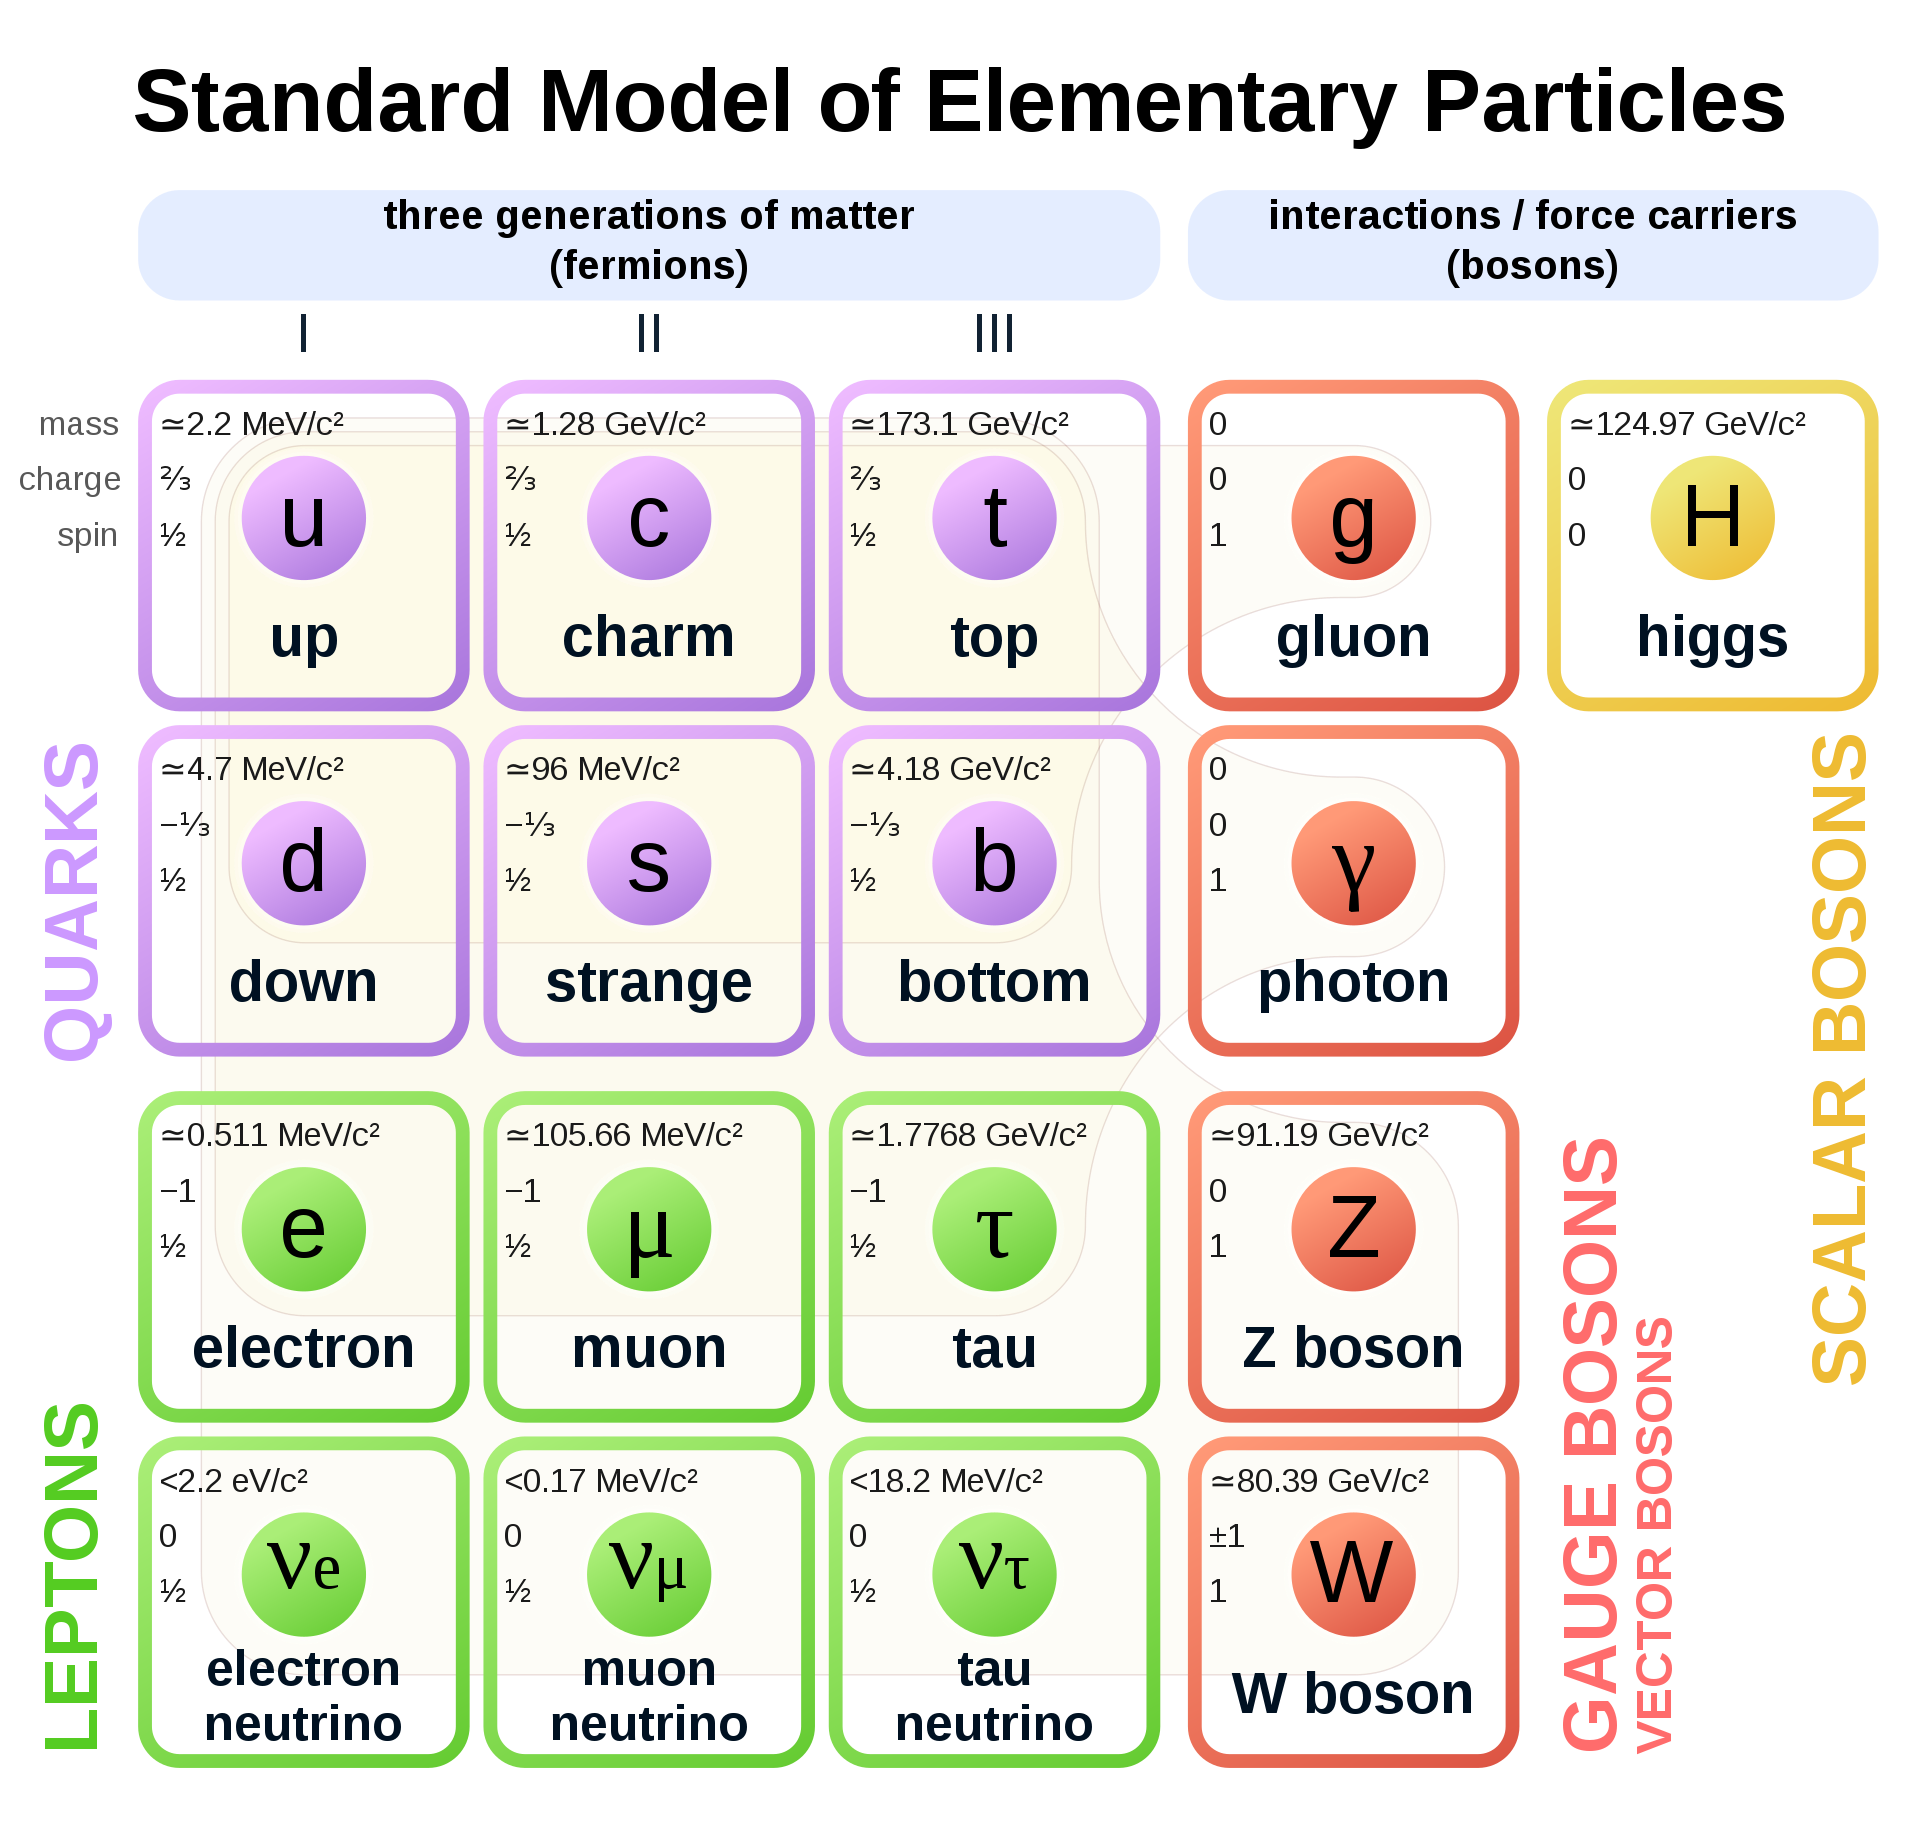
\includegraphics[width=\linewidth]{fig/standard_model.png}
    \captionof{figure}{standard model of particle physics}
\label{fig:standard_model}
    \end{center}
%\end{figure}

There are three different interactions which are mediated by bosons carrying spin 1.
The weak force exchange particles are the massiv $Z$ and $W^{\pm}$ bosons, the massless photons for the electromagnetic force and eight massless gluons are mediating the strong force. 
    In this experiment the $Z$ Boson is especially important. Its properties are shown in table \ref{table:zboson}:
    %\begin{table}
        \begin{center}
            \begin{tabular*}{\linewidth}{c c c}
        \toprule
                Charge & Mass \si{[MeV]} & $\Gamma$\si{[GeV]}\\%Decay Width \si{[GeV]} \\ 
        \midrule
                \small{0} & \small {$91.1876 \pm 0.0021$} & \small{$2.4952 \pm 0.0023$} \\
        \bottomrule
    \end{tabular*}
            \captionof{table}{Properties of the $Z$ Boson}
        \label{table:zboson}
        \end{center}
%\end{table}


\subsection{Drell-Yan Process}
A $Z$ Boson can be created during the so called ``Drell-Yan'' Process (fig. \ref{fig:drell_yan}). 

    \begin{center}
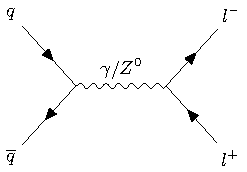
\includegraphics[width=0.7\linewidth]{fig/feynman_0.pdf}
        \captionof{figure}{Drell-Yan process}
\label{fig:drell_yan}
\end{center}

This process happens predominatly in proton-proton collisions.
When a quark and an anti-quark collide either a virtual photon $\gamma^\ast$ or a $Z$ Boson can be produced. 
The $\gamma^\ast$ or the $Z$ can then split into a lepton and its anti-particle partner like electron-positron or muon and anti-muon.
The sum of the lepton and anti-particle partner momenta will then add up to the former boson momentum. 
A peak around $90$ \si{GeV} will be observed corresponding to the $Z$ boson. 

\subsection{ATLAS Detector}
\subsubsection{Components}
The Detector consists of three main components: inner detector, calorimeters and the muon spectrometer.
They are onion-like constructed. 
The inner detector, the innermost layer, is mainly used to reconstruct the trajectories of electrically charged particles and to determine their momentum. 
With three aswell onion-like ordered tracking detectors, the pixel detector, the semi-conductor tracker and the transition radiation tracker, the inner detector can measure charged particles in a range of $\abs{\eta} < 2.5$ and a $p_{T} > 400$ \si{MeV}.\\

The electromagnetic and the hadronic calorimeter allow to reconstruct the shower shapes of the showers from electromagnetically and strongly interacting particles. 
They are designed to contain the whole shower and cover a range up to $\abs{\eta} < 4.9$. 
A precise energy measurement is possible.\\
The outermost layer is the muon spectrometer.
Muons would espace the ATLAS detector without it and can now be tracked. 

\subsubsection{Geometry of the detector}
In figure \ref{fig:cross_section_detector} one can see a drawing of the cross section of the ATLAS detector, which has a rotational symmetry around the $z$-axis.
A good understanding of the detector is necessary to compute the $Z$ bosons mass later on. 
One introduces the so called pseudo rapidity $\eta$:
\begin{align}
    \eta = - \log \tan \left( \frac{\theta}{2} \right)
\end{align}
The components of the momentum of a given particle are:
\begin{align}
    p_x = p_T \cos \phi \\
    p_y = p_T \sin \phi
\end{align}
where $p_T$ is the transversal momentum.
By using the $eta$ definition one can derive $p_z$ in the following way:
\begin{align}
    & p_z = p_t \cot \theta \\
    & \text{use: } \cot (2\arctan \e^{-x}) = \sinh x \\
    \Rightarrow \ & p_z = p_T \sinh \eta .
\end{align}
\begin{center}
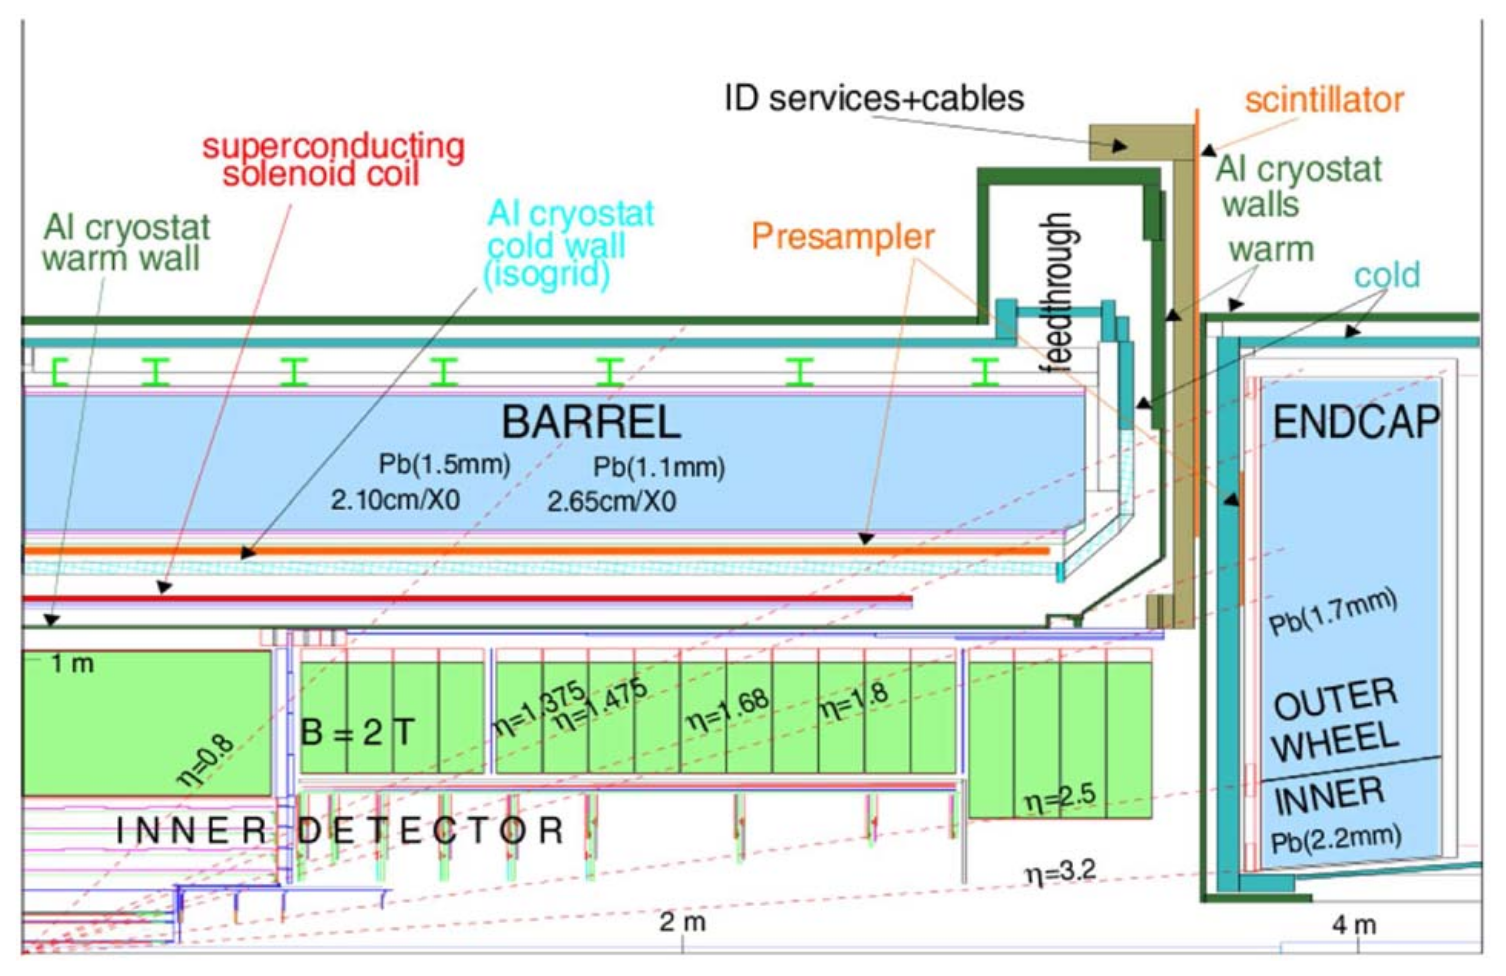
\includegraphics[width=\linewidth]{fig/detector_geometry.png}
        \captionof{figure}{Cross section of the detector}
\label{fig:cross_section_detector}
\end{center}

\subsection{Distributions}
For the experiment the following distributions are important.\\
Gaussian distribution:
\begin{align}
    f_{\text{G}} (E) = \frac{\mathcal{N}}{\sqrt{2 \pi \sigma^2}} \exp \left( - \frac{(E - \mu )^2}{2 \sigma^2} \right)
\end{align}
Breit-Wigner Distribution:
\begin{align}
    f_{\text{BW}} = \frac{\mathcal{N} k}{(E^2 - M^2)^2 + M^2 \Gamma^2} ,
\end{align}
with $k = \frac{M\Gamma \gamma \sqrt{8}}{\pi \sqrt{M^2 + \gamma}}$ and $\gamma = M \sqrt{M^2 + \Gamma^2}$. $Gamma$ is the decay width.\\
One also needs a third distributions which is the convolution of the Gauss and the Breit-Wigner Distribution in order to account for the uncertainties caused the detector.
The Breit-Wigner describes the physical decay process. 
However it does not consider the energy uncertainties which can be recognized by the gaussian distribution.
A convolution of two functions $(f \ast g)$ is defined as:
\begin{align}
    (f \ast g) (x) = \int f(y)g(x-y)\dd y
\end{align}

\subsection{Efficiency}

The efficiency of the measurements plays a crucial role. 
At the ATLAS detector it consists of for components:
\begin{align}
     \epsilon_{\text{tot}} =  \epsilon_{\text{recon}} \times \epsilon_{\text{id}} \times \epsilon_{\text{trig}} \times \epsilon_{\text{add}} 
\end{align}
The focus on this experiment lies on the identification efficiency.
One can get an estimate for $\epsilon_{\text{id}}$ by using the so called tag and probe method.
One searches for one event where two electrons are involved. 
Now strict conditions are applied on one of the electrons, the \textit{tag} electron, 
and on the other one, the \textit{probe} electron, weaker conditions are applied.
Let $N_tp$ be the number of events where both tag and probe fulfill their conditions and $N_t$ be the number of events where only the tag electron passes the requirements, then the efficiency is given by:
\begin{align}
    \epsilon_{\text{id}} = \frac{N_tp (p_T)}{N_t(p_T)}.
\end{align}


\section{Experimental procedure}

\subsection{Getting familiar with the data}
Before starting with the computation of the mass of the $Z$ bosons one has to make oneself familiar with the provided data of the ATLAS detector and the data analysis library \verb*+ROOT+.
The given data was preselected; one only has data from events where a primary vertex was found and at least one lepton has a minimal transverse momentum of $p_{T} = 25$ \si{GeV}.

\subsubsection{Particle entrance}
\begin{center}
	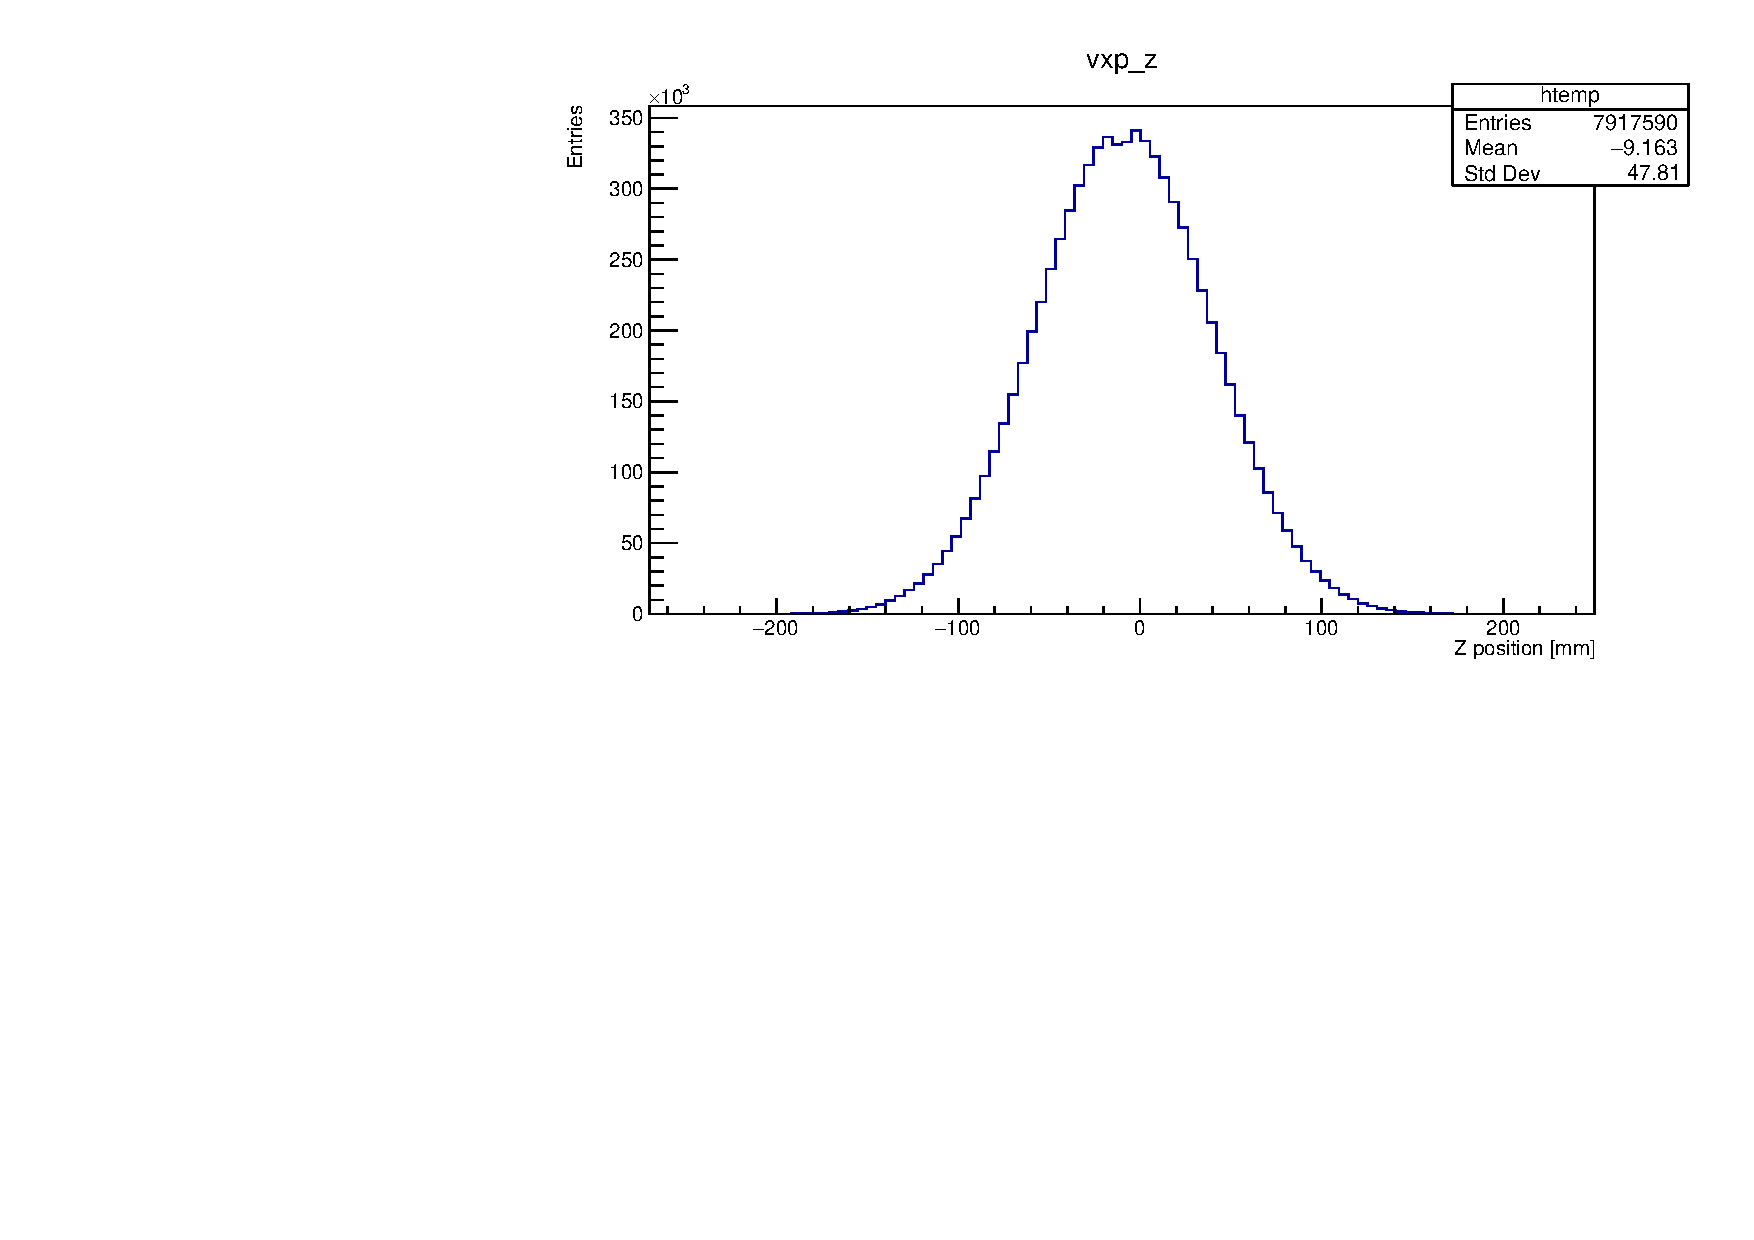
\includegraphics[width=\linewidth]{fig/vxp_z_redo.pdf}
    \captionof{figure}{$z$-postion distribution, particle entrence in ATLAS detector}
	\label{vxp_z}
\end{center}
To check where the particle enter the detector, one can evaluate the given date for the vxp\_z variable. 
The results are shown in fig. \ref{vxp_z}.
The mean is shifted for $-9$ \si{mm}. 
This confirms, that the given data is from 2012 because collisions of bunches were not calibrated to the $0.0$ position back then \cite{atlasbeamspot}.
Left and right to the mean are two maxima, which can also be explained with the assumption above. 
A momentum change of $90$ degrees is impossible and most of the collisions take place at the place of the first intersection.

\subsubsection{leptons per event}

\begin{center}
	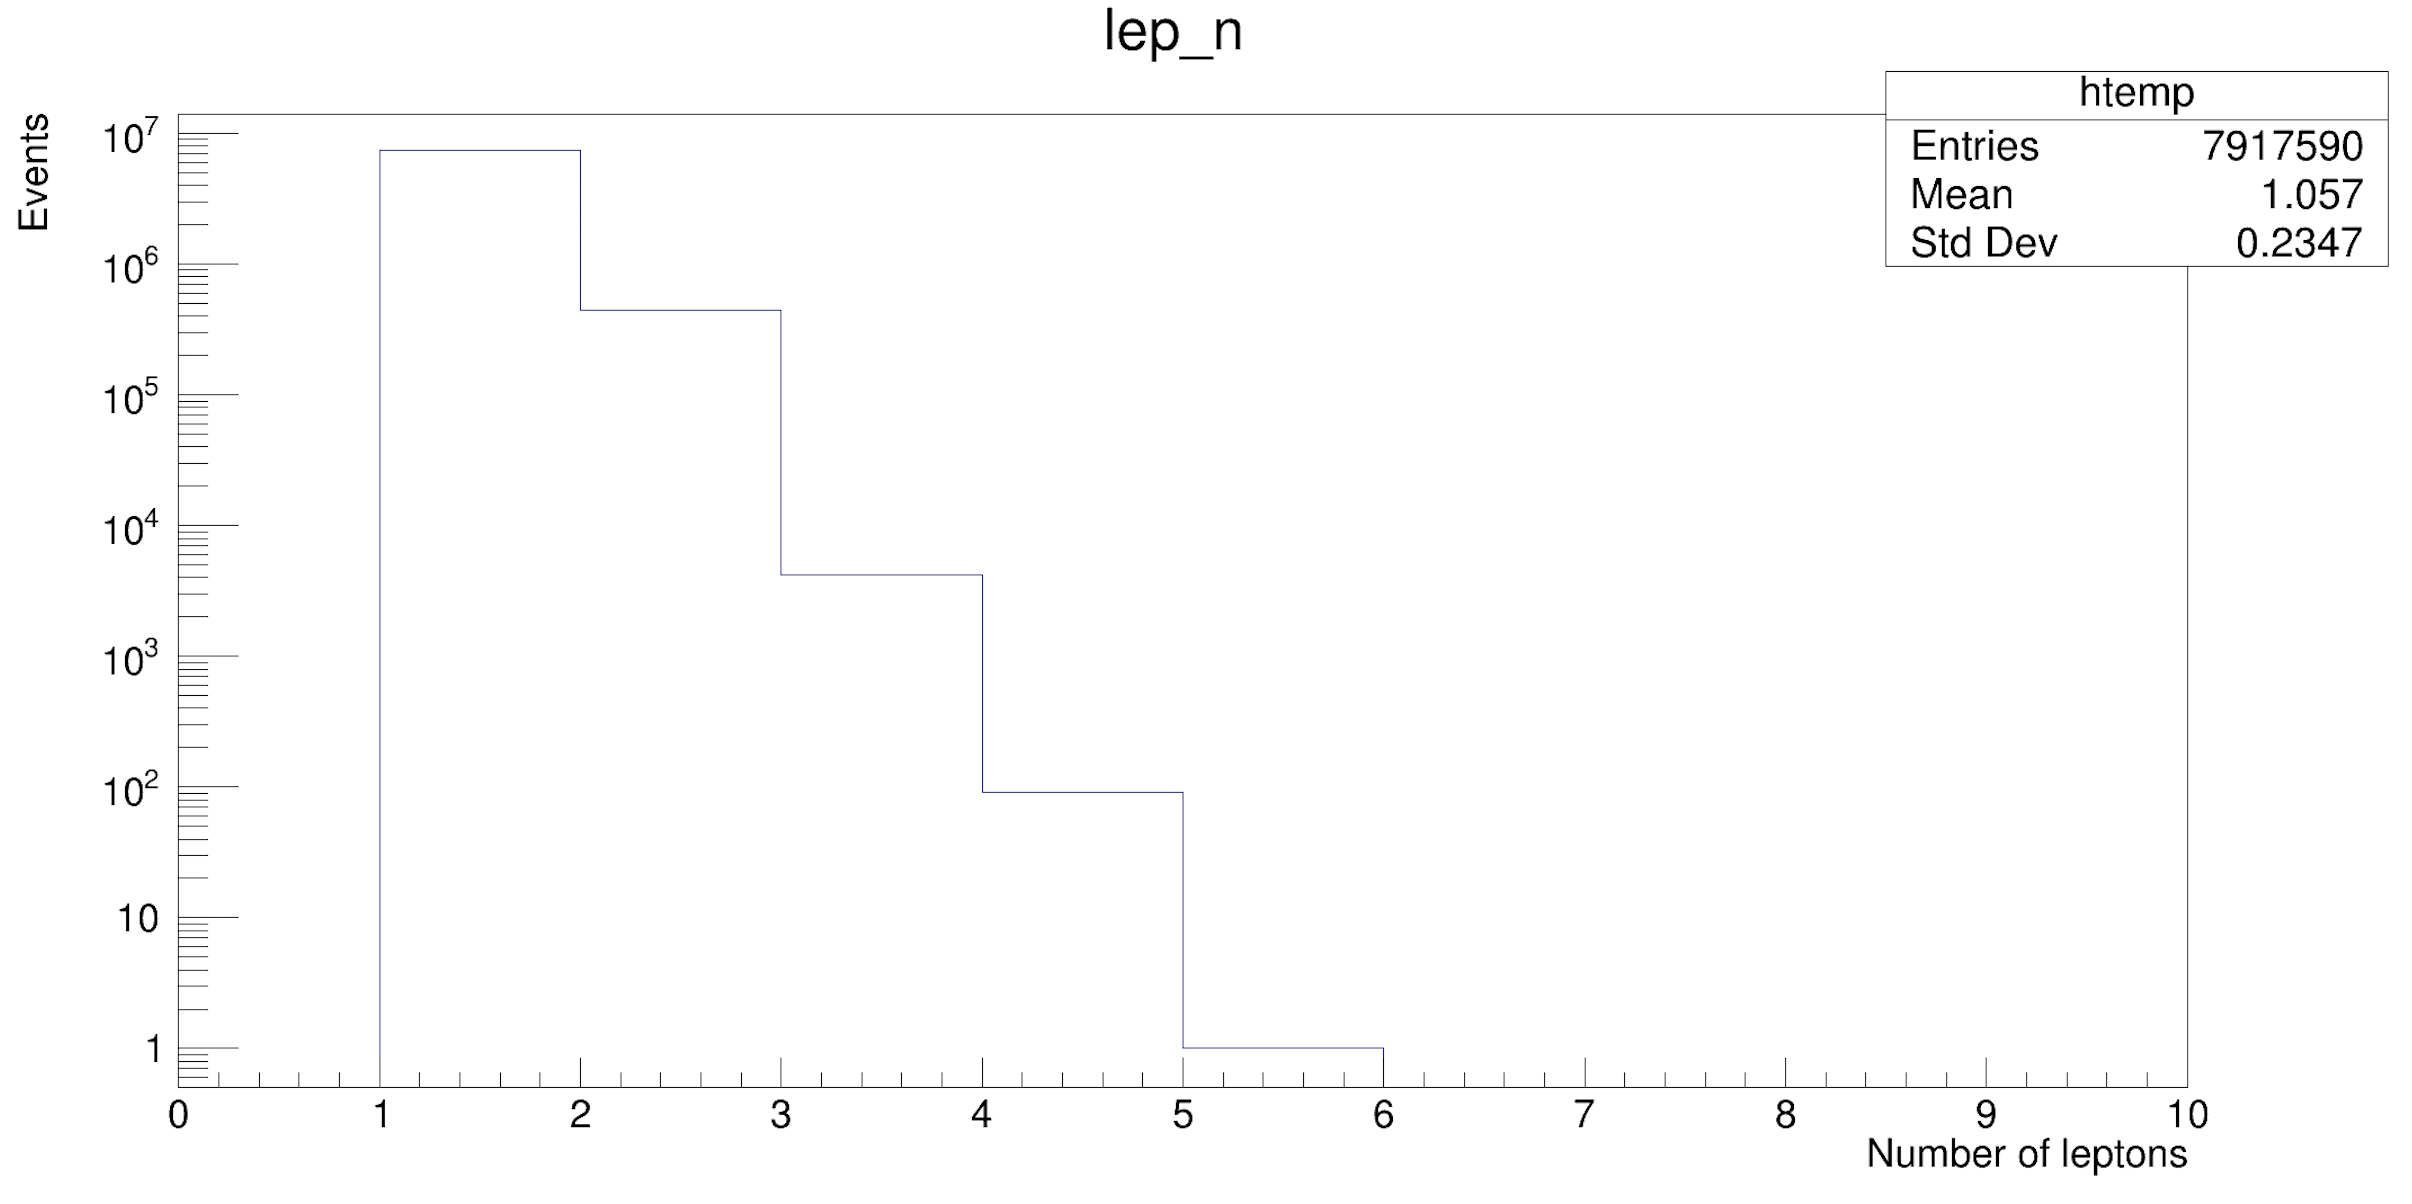
\includegraphics[width=\linewidth]{fig/number_produced_leptons.png}
    \captionof{figure}{leptons recorded per event}
	\label{lep_n}
\end{center}

To figure out, if one found a $Z$ decay, one analysis the \textit{leptons per event} value of the data (fig. \ref{lep_n}).
Around the wanted two leptons, one gets many events with one and three leptons. 
For these events to happen, one needs a $W^{\pm}$ decay.
Possible decays are shown in \ref{fig:three_lepton}
    \begin{center}
        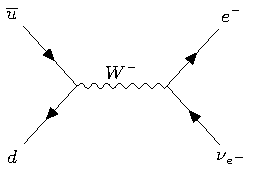
\includegraphics[width=0.45\linewidth]{fig/feynman_1.pdf} \hfill
        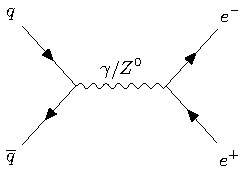
\includegraphics[width=0.45\linewidth]{fig/feynman_2.pdf} \\
        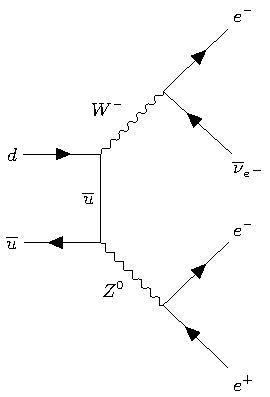
\includegraphics[width=0.45\linewidth]{fig/feynman_3.pdf}
\captionof{figure}{Feynman graphs for final states with one to three leptons}
\label{fig:three_lepton}
\end{center}

\subsubsection{Data of the leptons}
The stored data about transvers impuls, the $\phi$ degree and $\eta$ varible provide information about all the leptons recorded by the ATLAS detector and accordinlgy has more entries than the former analyzed data variables.
\begin{center}
    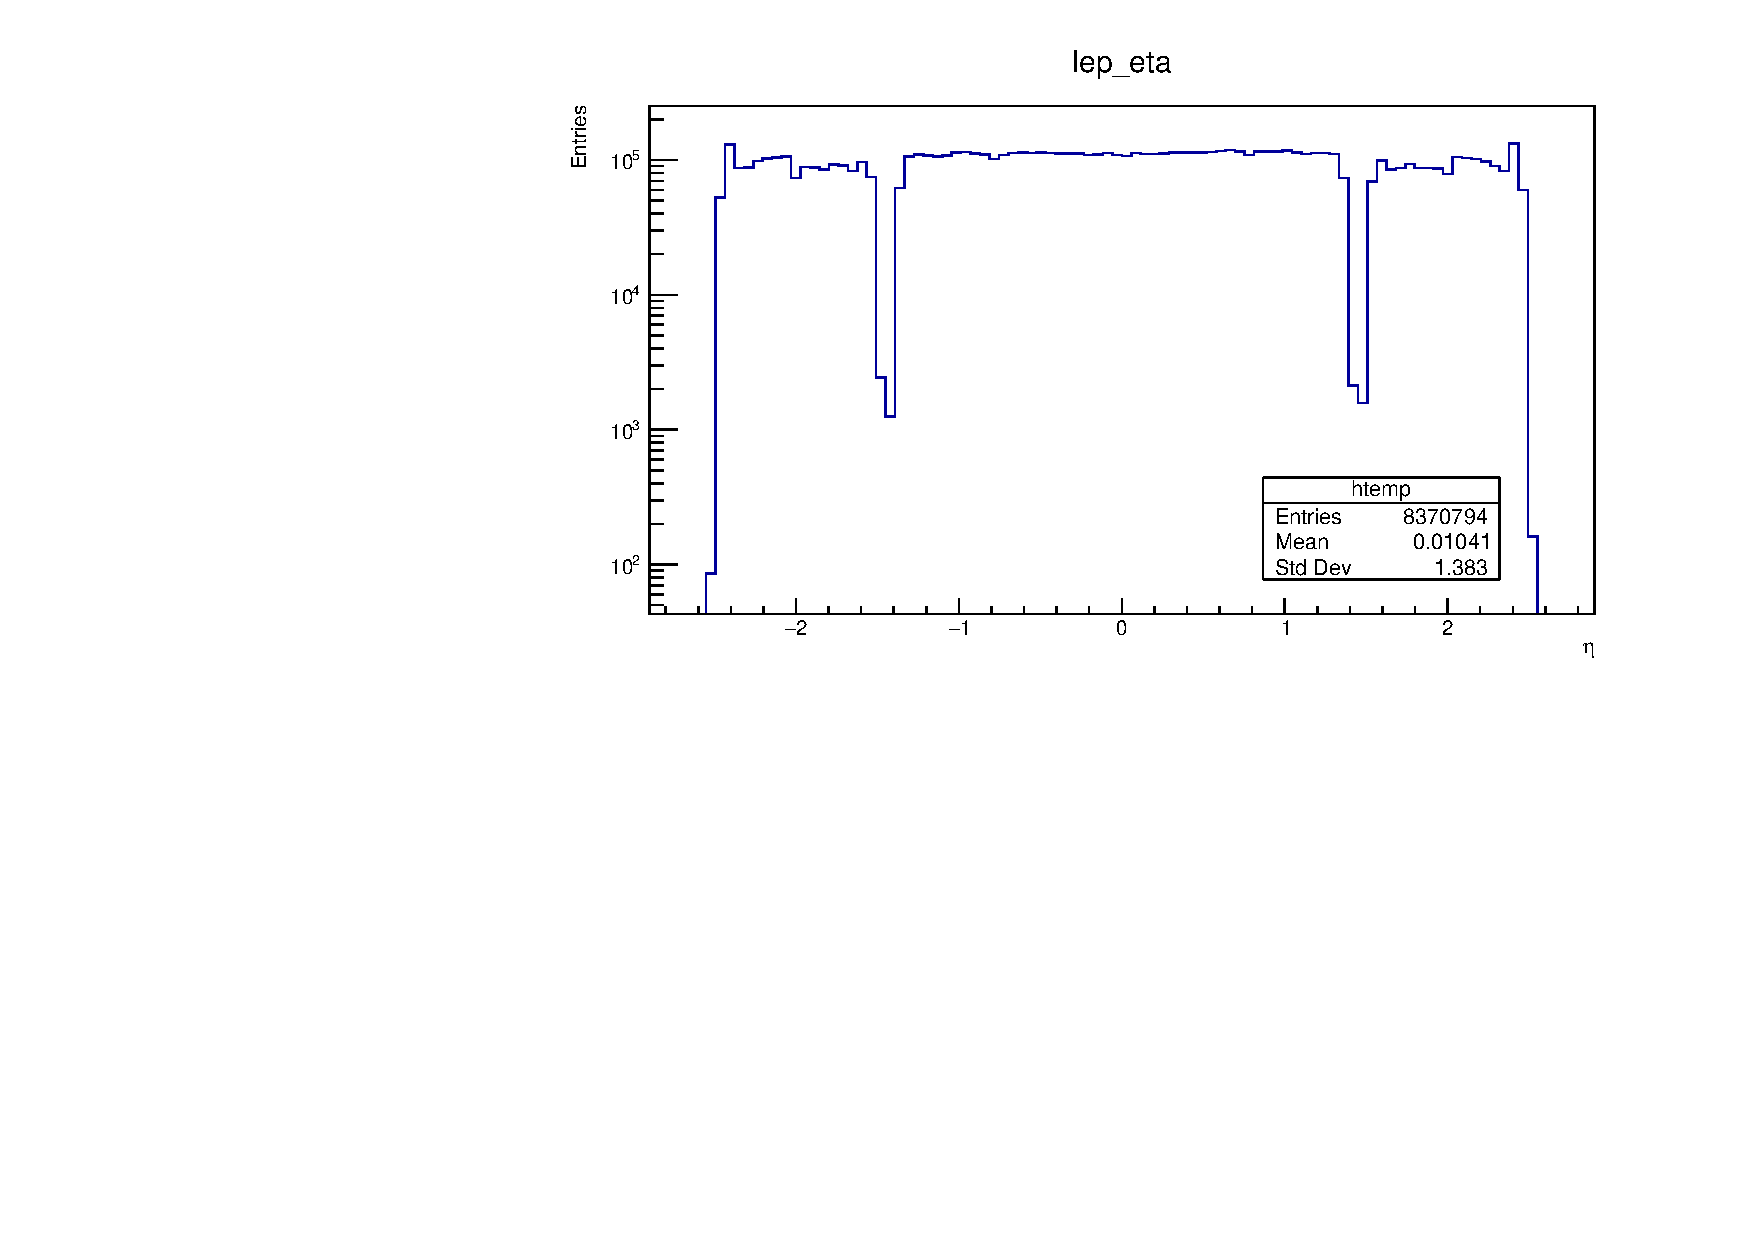
\includegraphics[width=\linewidth]{fig/lep_eta_redo.pdf}
    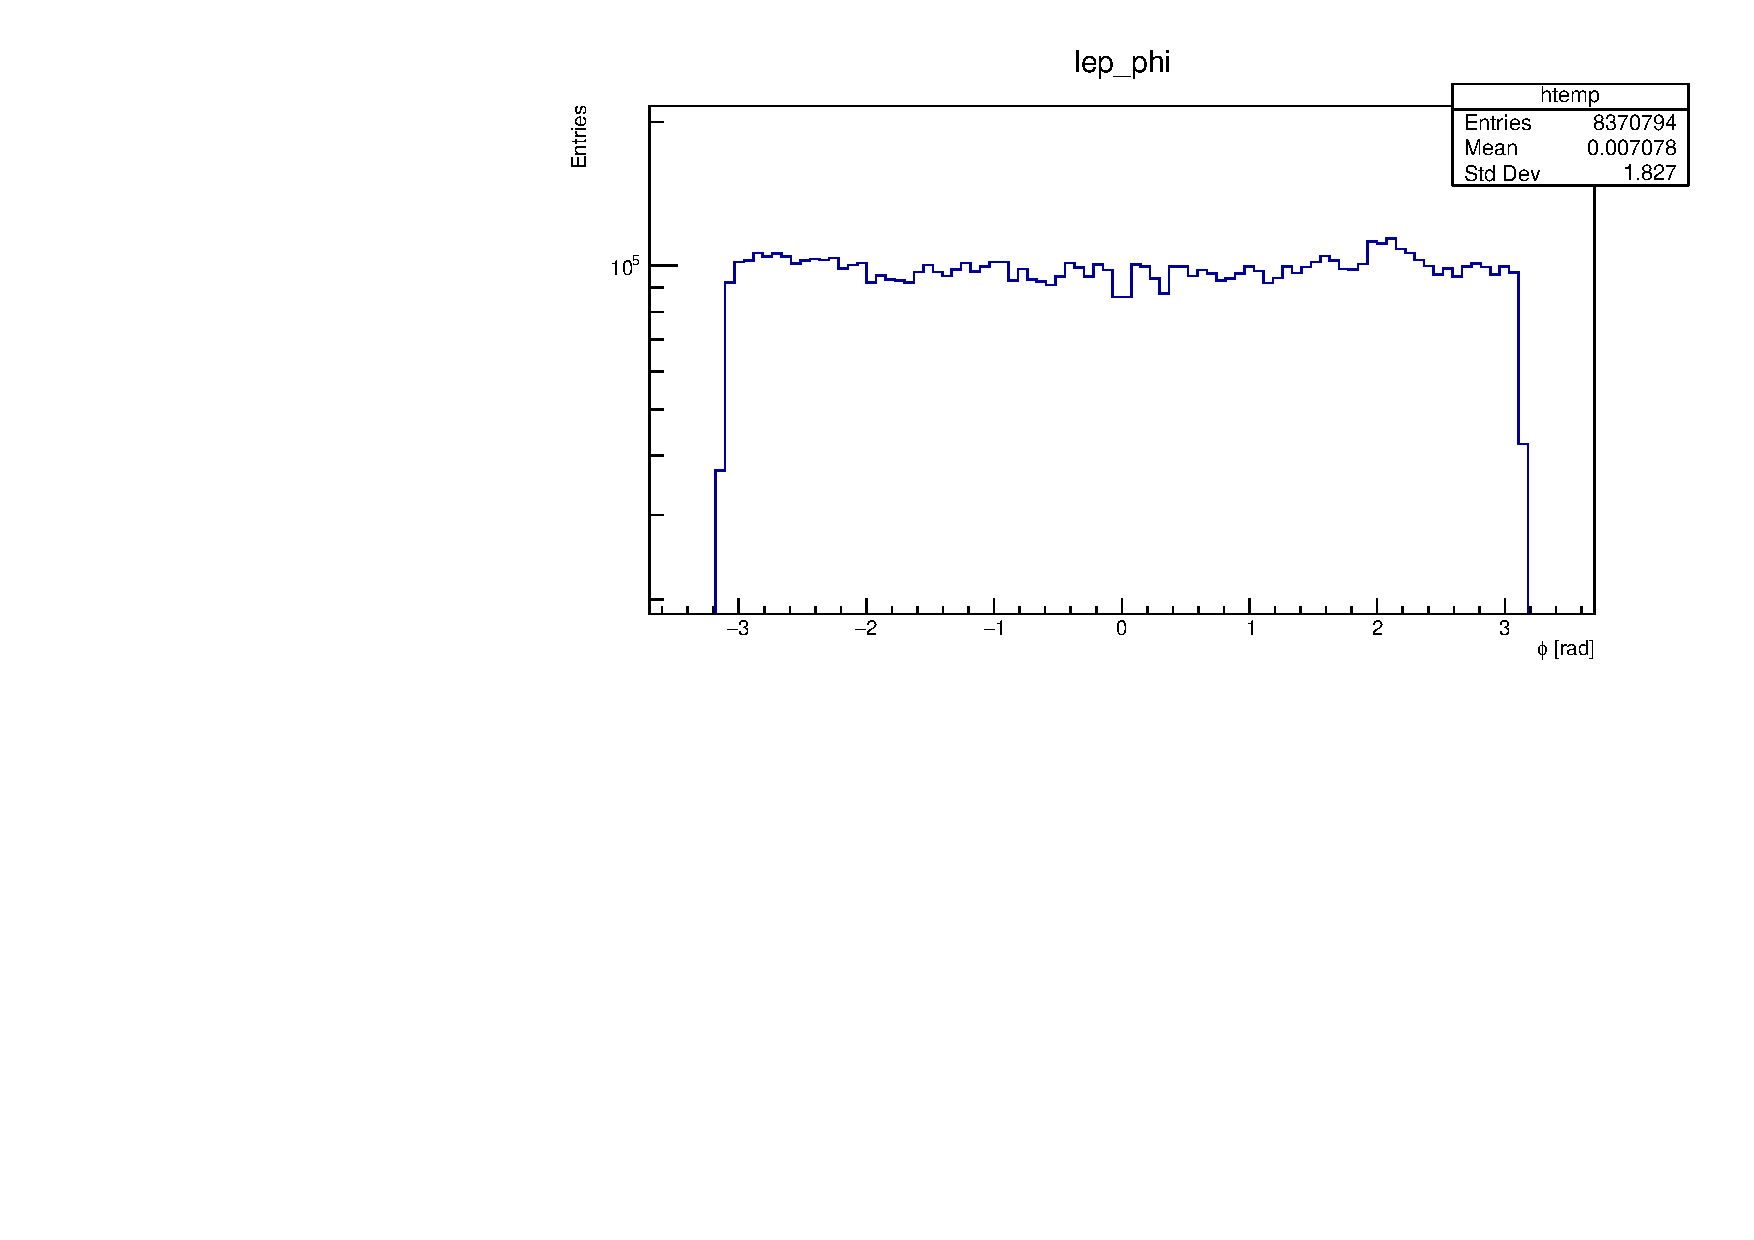
\includegraphics[width=\linewidth]{fig/lep_phi_redo.pdf}
    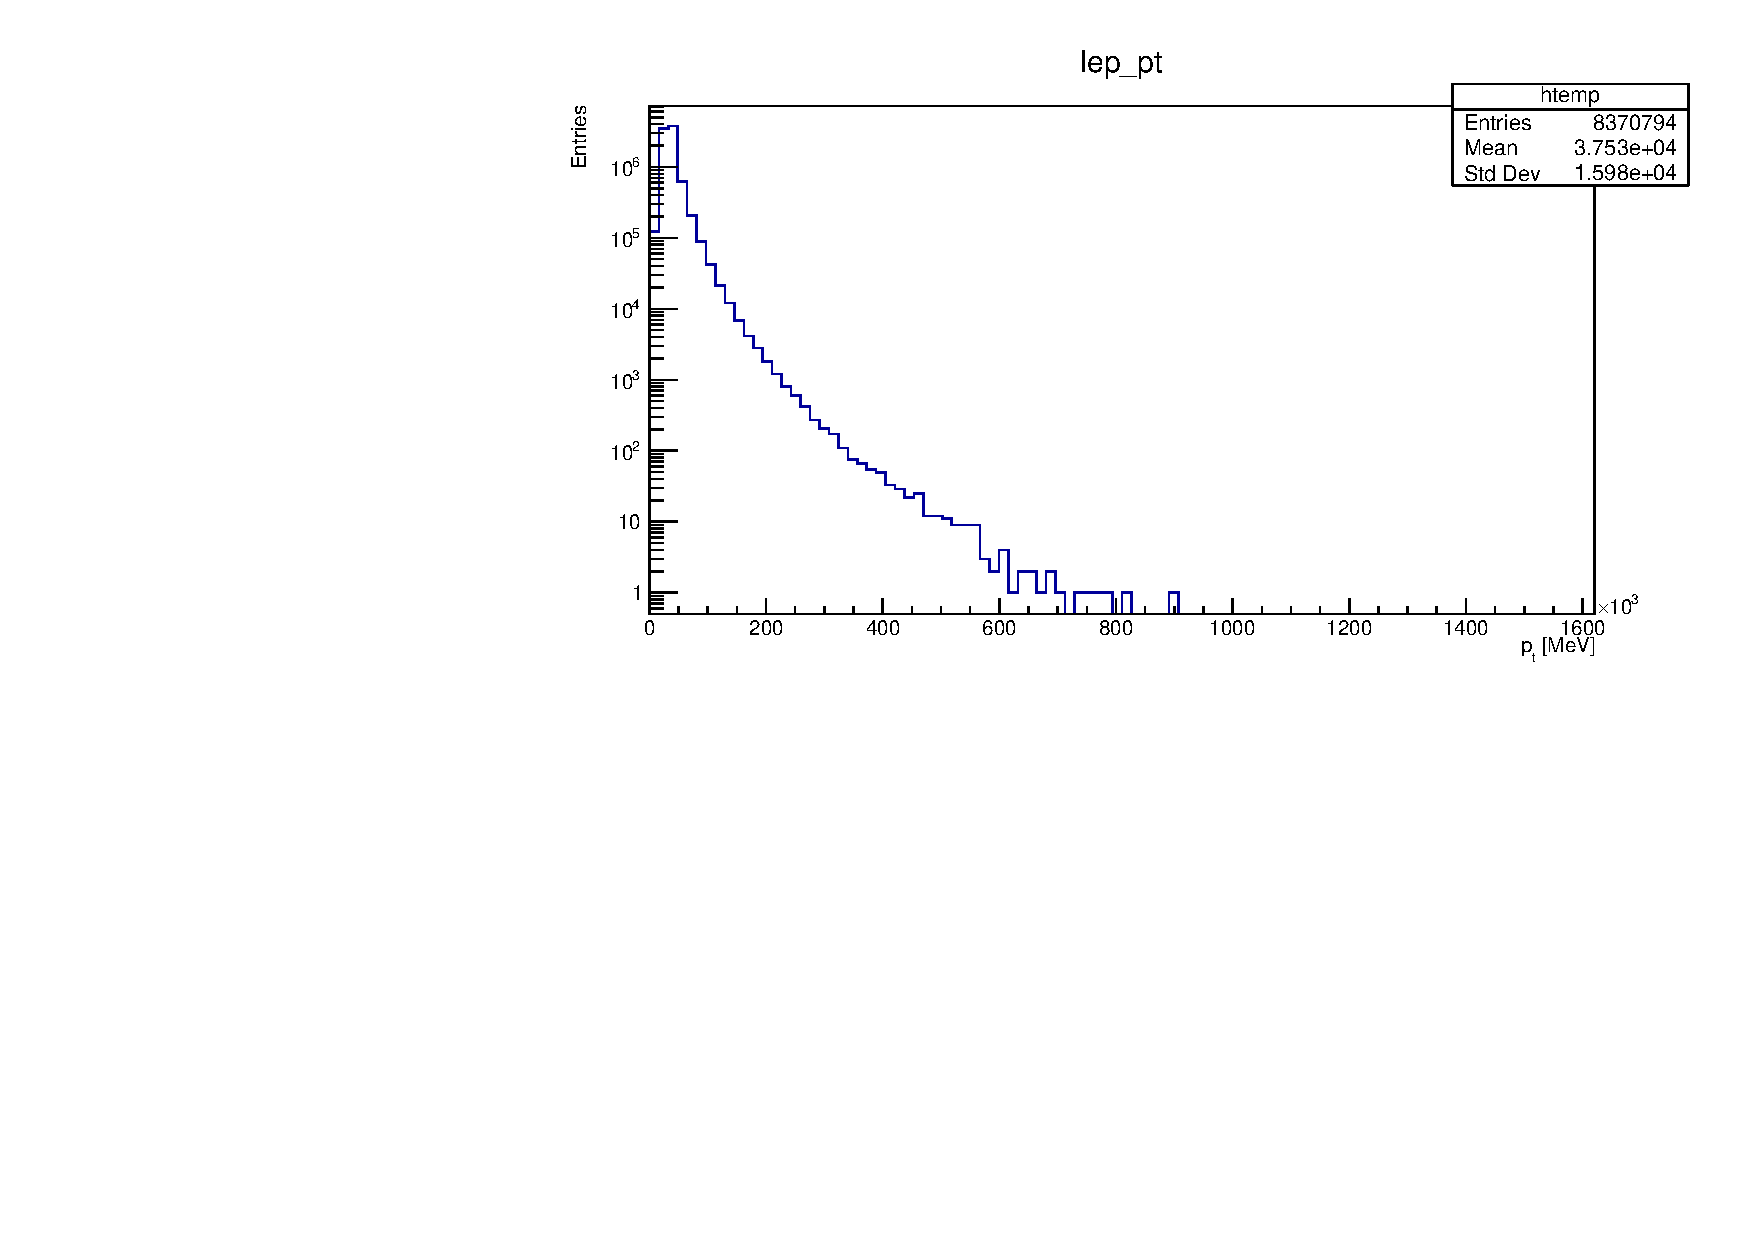
\includegraphics[width=\linewidth]{fig/lep_pt_redo.pdf}
    \captionof{figure}{Distributions of $\eta$, $\phi$ and $p_t$}
\end{center}


\subsection{Calculation of the invariant mass of the $Z$ boson}
According to the structure of the ATLAS detector, one can calculate the invariant mass in the following way:

\begin{align}
	M_{\mu} &= \sqrt{p_{\mu}p^{\mu}} = \sqrt{E_{1}E_{2}-\vec{p_{1}}\vec{p_{2}}}%\\
			%&= \sqrt{E_{1}E_{2}-p_{T_{1}}p_{T_{2}} (\cos(\varphi_{1})\cos(\varphi_{2})+\sin(\varphi_{1})\sin(\varphi_{2})+\sinh(\eta_{1})\sinh(\eta_{2}))}
\end{align}


An attempt to calculate it with the above given formula and the build-in function \verb*+TLorenz+ in \verb*+ROOT+ provided the exact same result. 
The calculated results will therefore be based on the \verb*+ROOT+ method.


The first attempt to measure the mass was done by limiting the data to 2-lepton events. 
Further one ignored the events where $M_{\mu}^{2} < 0$. 
\begin{center}
	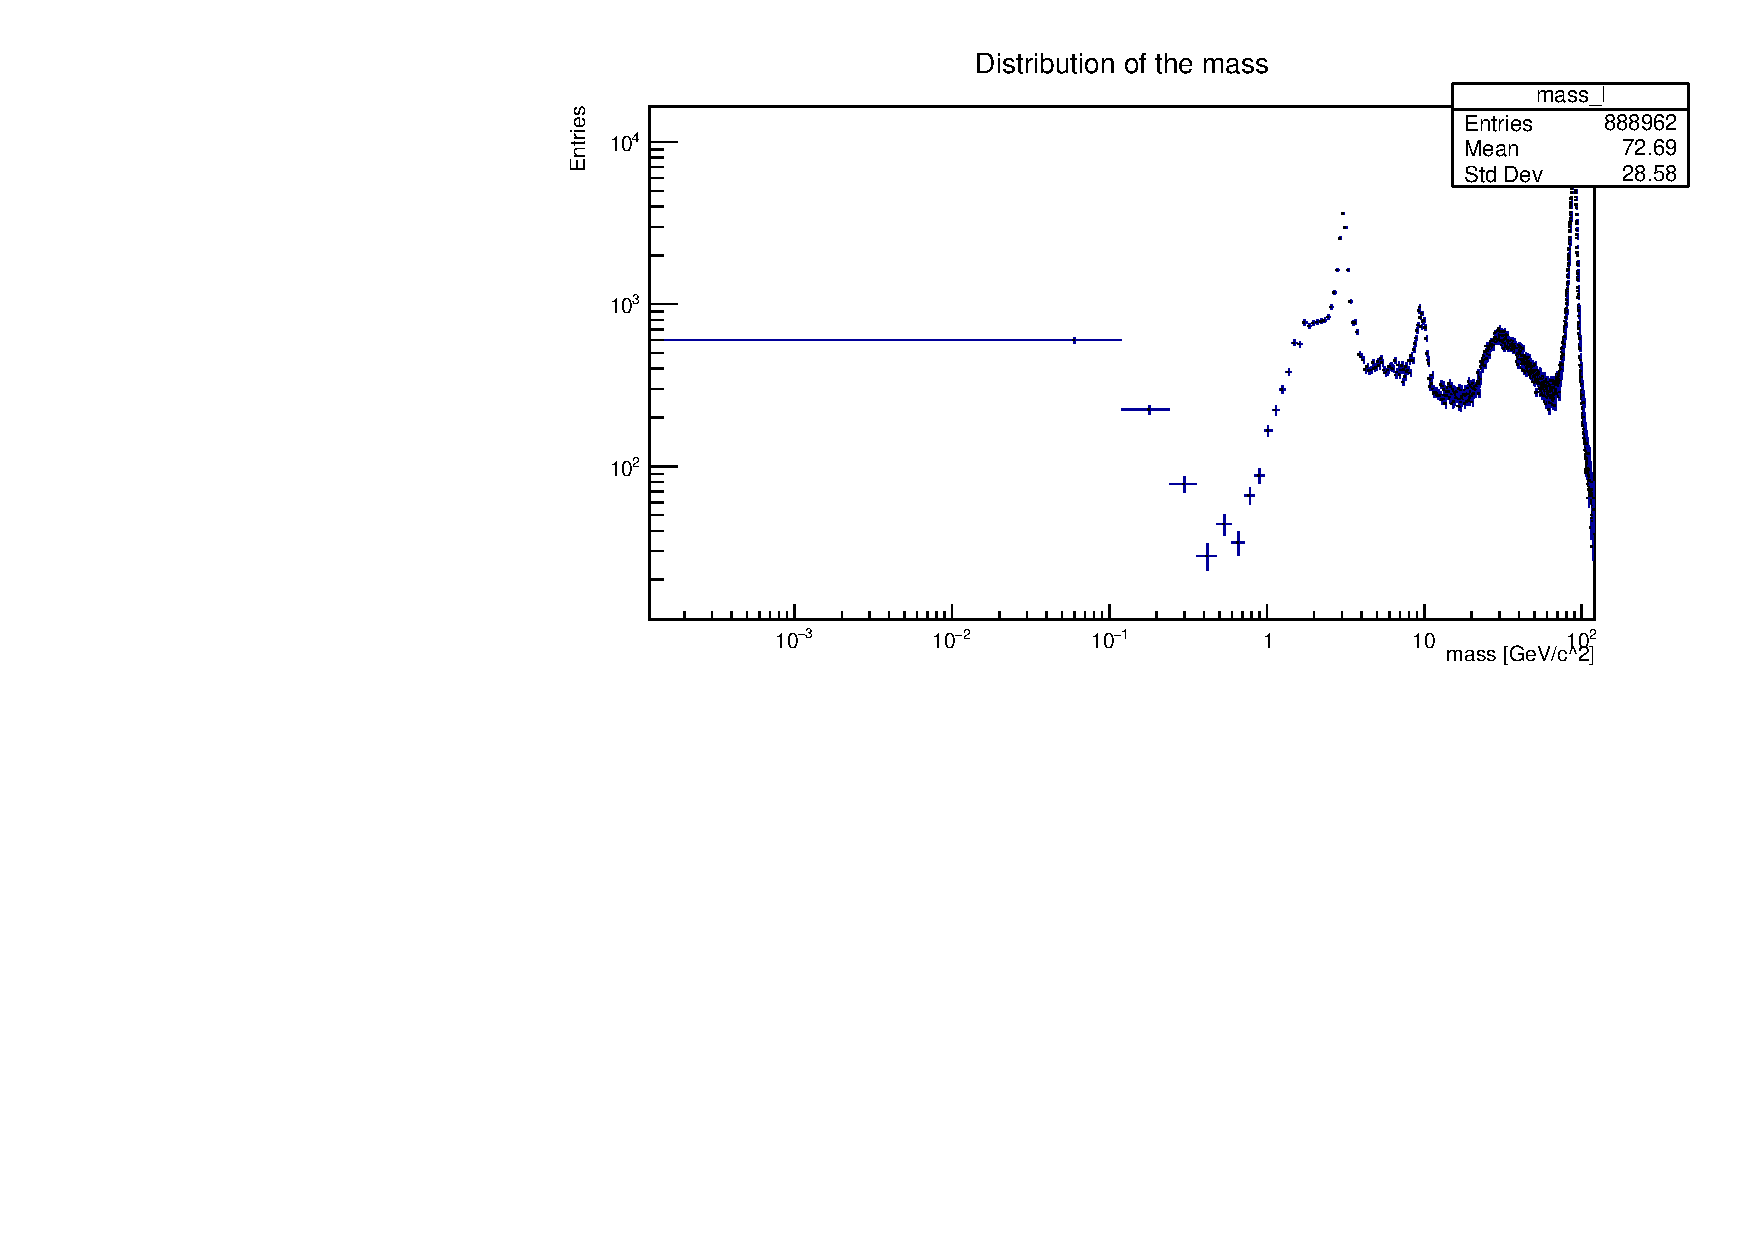
\includegraphics[width=\linewidth]{fig/mass_lz_log.pdf}
    \captionof{figure}{invariant Mass distribution of 2 lepton events}
	\label{mass_lz_log}
\end{center}

In ~\ref{mass_lz_log}, one can identify four peaks. 
The one on the right, at approximatly $91$ \si{GeV}, is the subject of this investigation and the goal is to characterize it better in the course of this paper.\\
The two on the left are respectable by the virtue of the $J/{\Psi}$ and the $\Upsilon$ decay. 

\subsection{Selecting} 
The next step was to assert restictions to the dataset in order to ensure that a $Z$ decay was meassured.
The impact of each of the restrictions can be seen in fig.\ref{fig:cutflow}. 
\begin{center}
	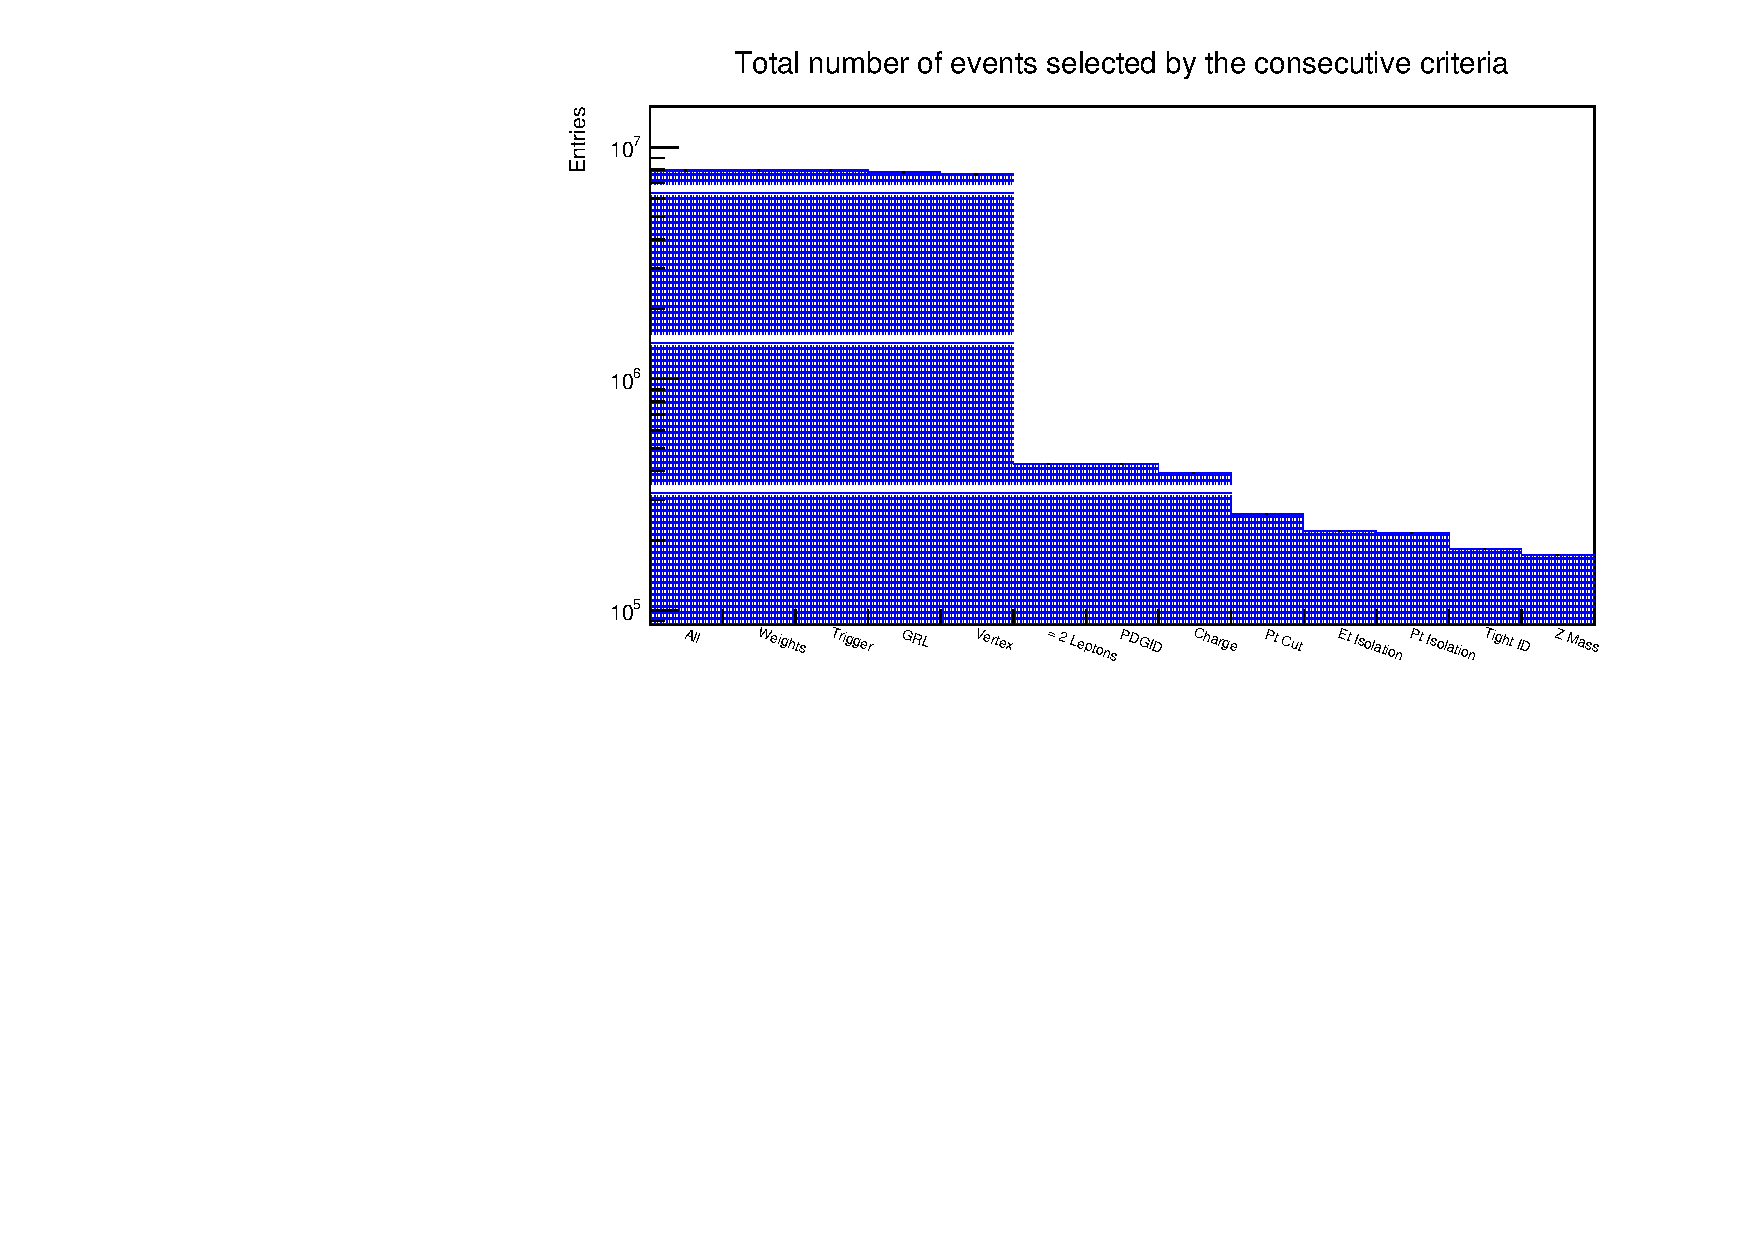
\includegraphics[width=\linewidth]{fig/cutflow.pdf}
    \captionof{figure}{cutflow histogramm}
	\label{fig:cutflow}
\end{center}
The eventbased cuts (in fig.\ref{fig:cutflow} the first four columns) have close to no impact on the selection because the given raw data from ATLAS is preselected on event and physics object level.
As seen, the highest cut impact provides the 2 lepton cut, which  is necessary for a $Z$ decay. ATLAS only required one well measured primary vertex to save it as an event.
The cut with the second highest impact is the $p_{T}$ Cut. Due to the high mass of the $Z$ Boson, one can restrict oneself to leptons with at least $25$ GeV. The distribution of the transvers momenta from the two decay leptons peaks around half the $Z$ mass. 


\subsection{Comparing Data and MC Simulation}
One can now ask how well the meassured data matches with the theory. 
In order to do this one can do MC Simulations and then compare with the data (fig. \ref{fig:data_mc}). Three MC simulations for the possible leptons after the $Z$ decay are analysed in the same way as in section 2.3 explained. One has to scale the results according to the luminosity of the ATLAS detector ($1 fb^{-1}$).
The comparison yields matching results.

\begin{center}
	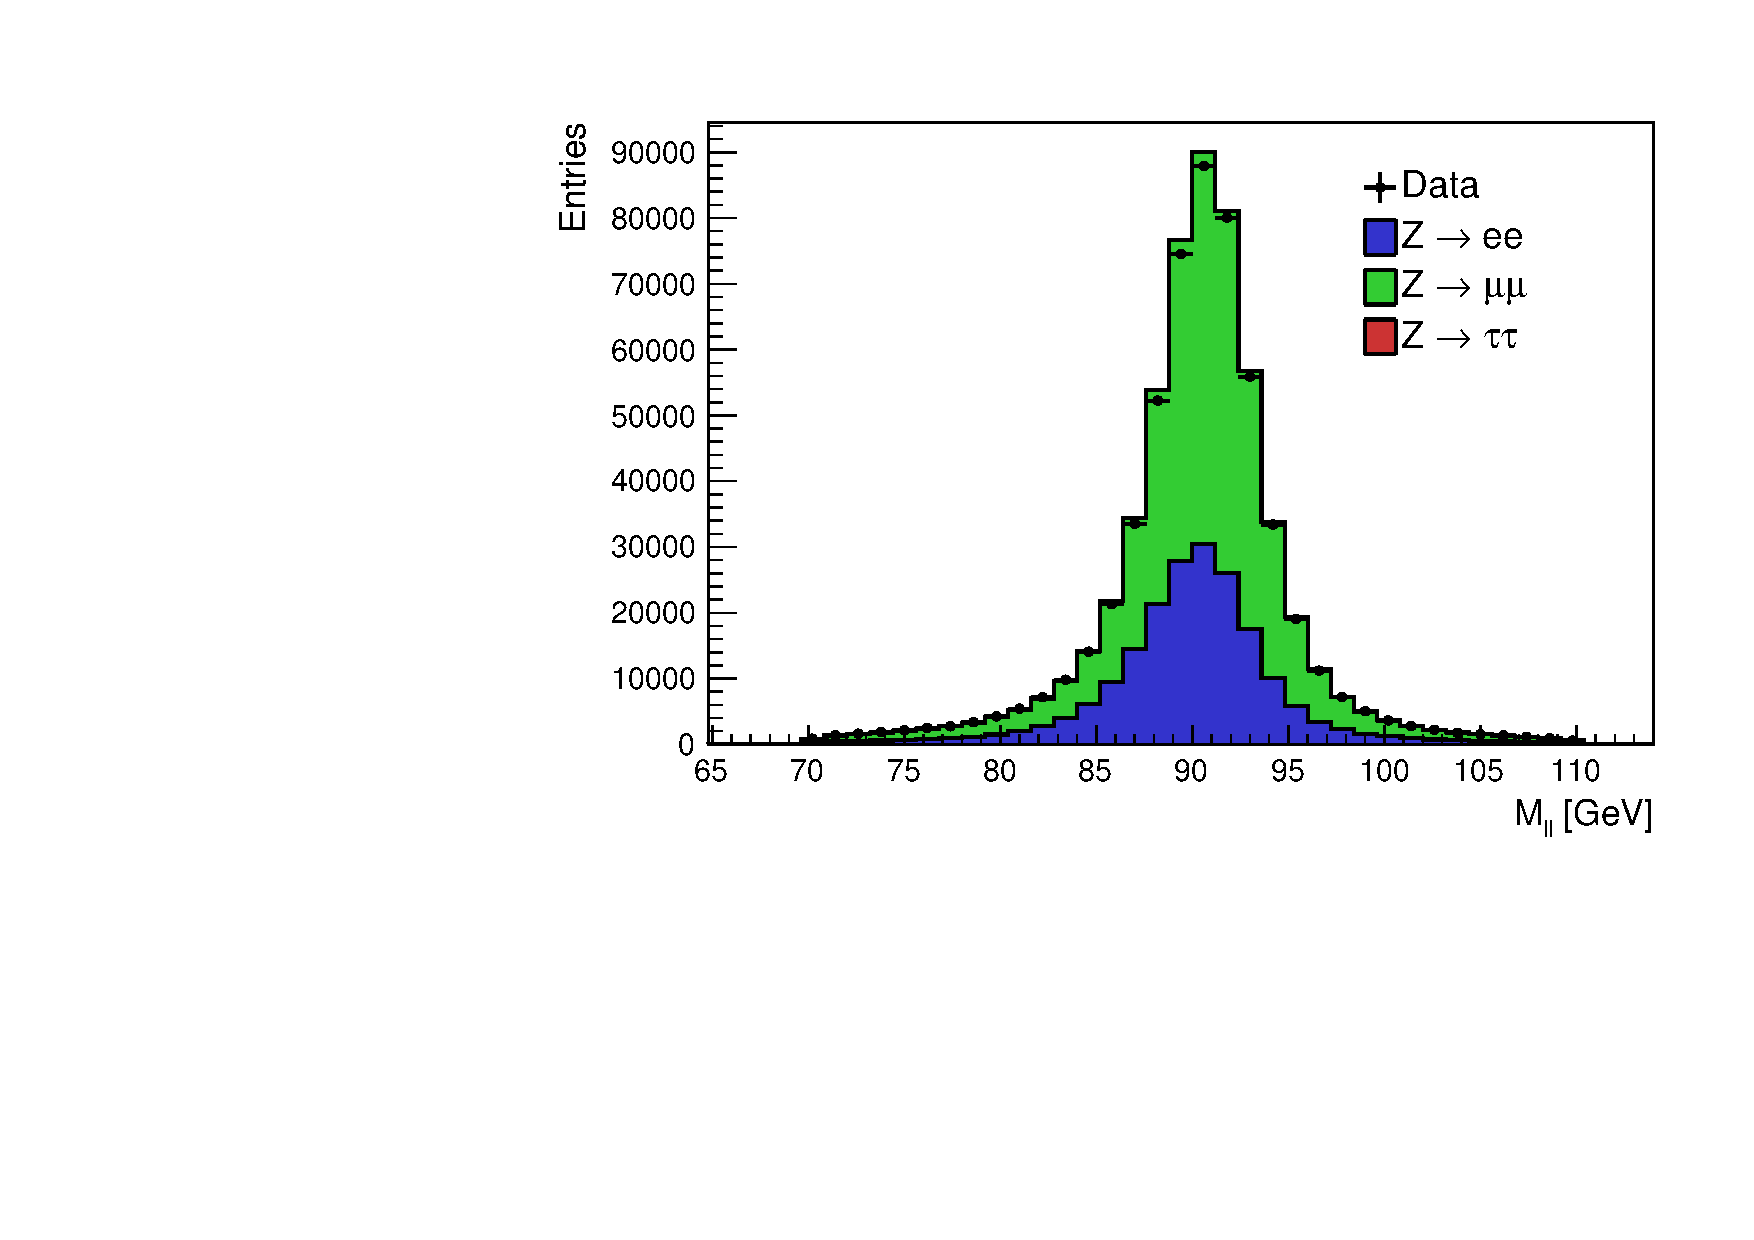
\includegraphics[width=\linewidth]{fig/vergleich_data_mc_final.pdf}
    \captionof{figure}{Comparison of meassured data and MC simulation}
	\label{fig:data_mc}
\end{center}

\subsection{Fitting the $Z$ mass}
The best fit can be achieved by computing a convolution of a Gauss and a Breit-Wigner Curve.
The reason is the Doppler effect (?)

\begin{center}
	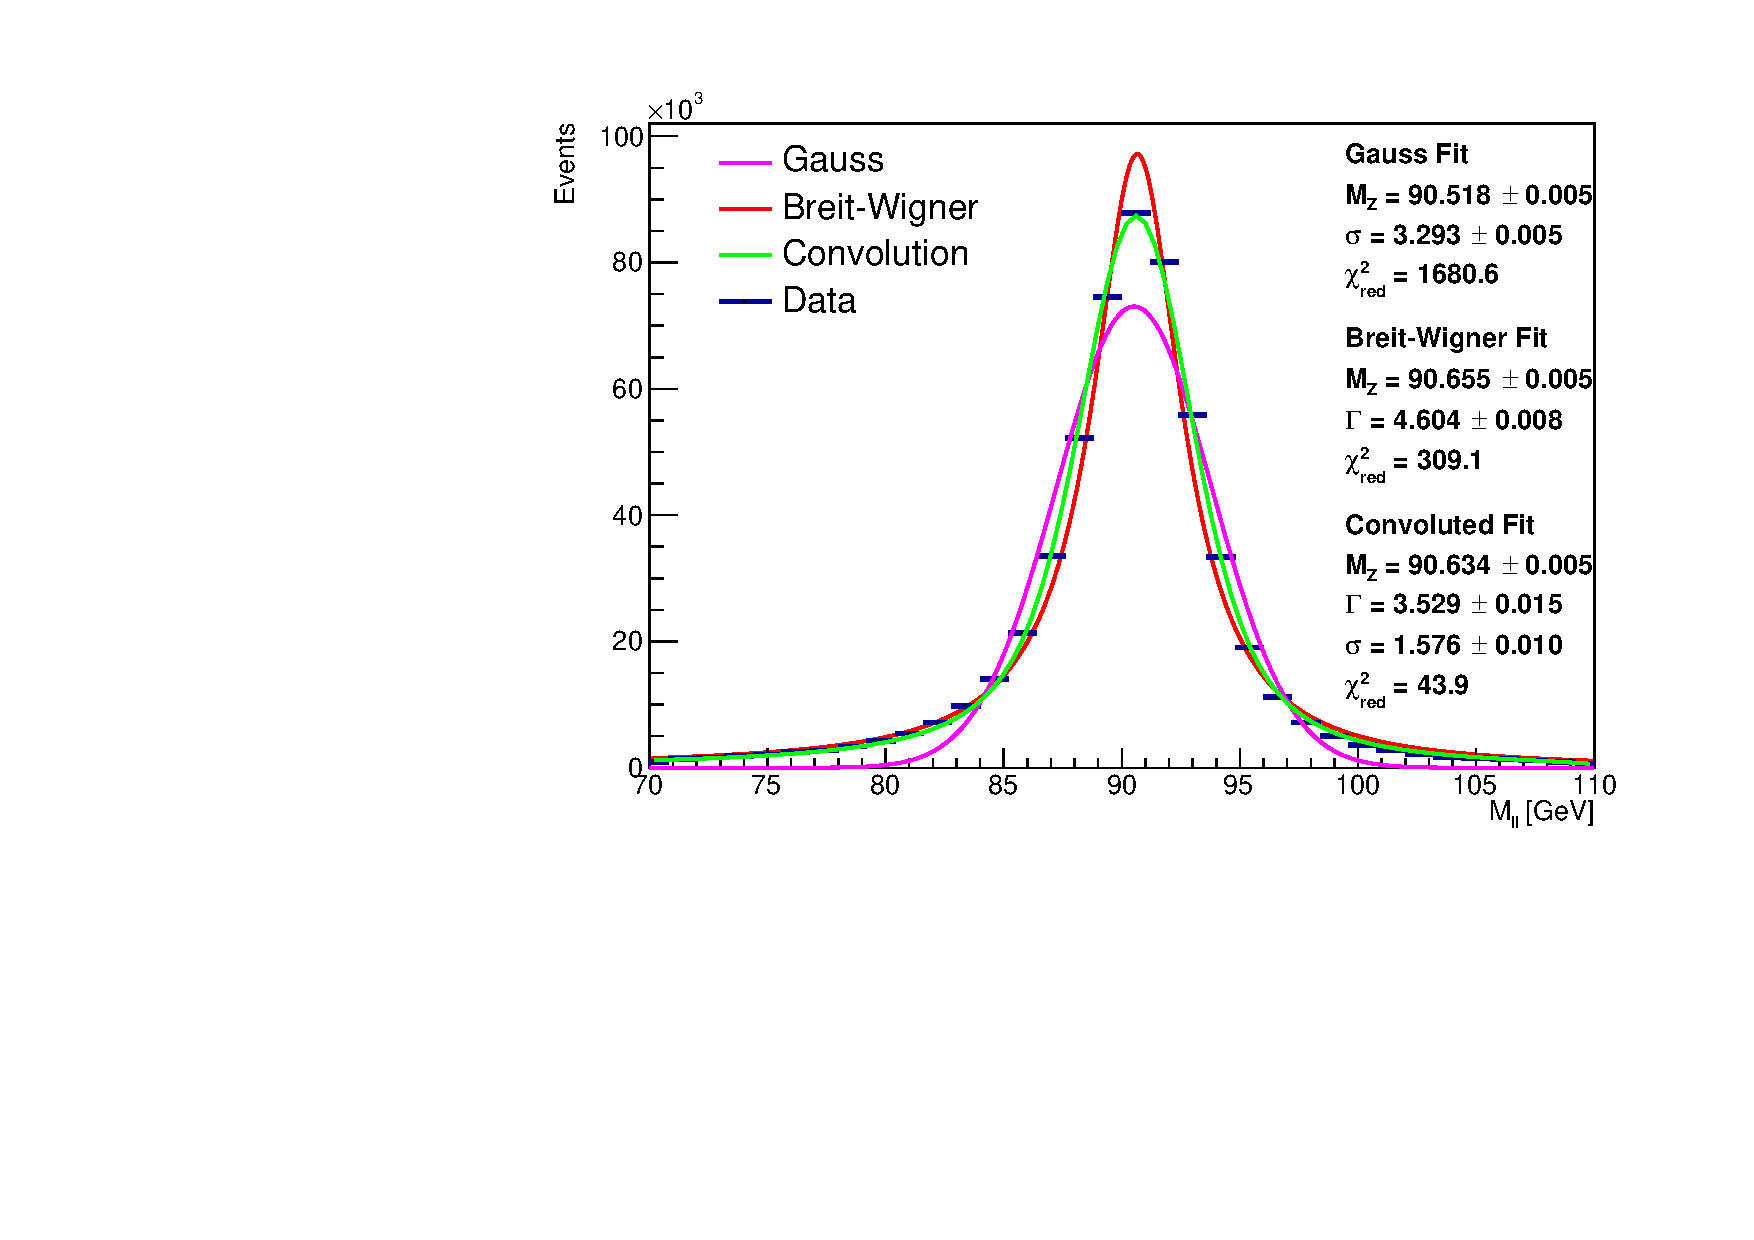
\includegraphics[width=\linewidth]{fig/invar_z_mass.pdf}
    \captionof{figure}{Comparison of meassured data and MC simulation}
	\label{fig:fit}
\end{center}


\subsection{Determining efficiencies}
For determining the efficiency of the identification the tag and probe method (which was introduced earlier) is used.
The efficiency was computed for the MC-Simulation and for the real data and can be seen in figure \ref{fig:efficiency_comp}

\begin{center}
    \includegraphcis[width=\linewidth]{fig/efficiency_comparison.pdf}
    \caption{figure}{Comparison of the efficiencies of the MC-simulation and the real data}
    \label{fig:efficiency_comp}
\end{center}


\section{Discussion}

\subsection{Systematic errors}

\section{}

\nocite{*}
\appendix
\printbibliography
\end{multicols}
\end{document}



